\section{Results}
\label{section:results}

In this section we discuss the results of the experiments described in the previous section.


\subsection{Result 1. Toponym Resolution}

\begin{figure}
    \centering
    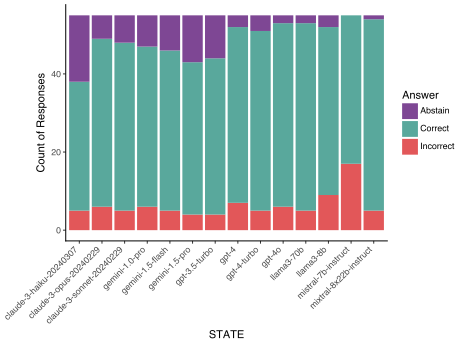
\includegraphics[width=\columnwidth]{figures/toponym_bar_state}
    \caption{The results of the toponym experiments show that most models resolve most toponyms to Australia. We filter out the `confusing' toponyms for subsequent experiments}
    \label{fig:toponym}
\end{figure}

The toponym experiments shown in figure~\ref{fig:toponym} shows report scores $>0$ as 'correct', $0$ as `incorrect' and `abstain' when the model returned `ICATQ'. 
Most models are capable of answering toponym resolution questions, with the majority of abstains associated with indigenous place names. 
Mistral-7b produced excessive tokens when answering questions, contributing to its increased error rate, whereas gpt-4 resolved toponyms like `Port Arthur', `Exmouth' and `Roma' to Texas, the United Kingdom and Italy respectively.
These are valid resolutions, but were useful for identifying places that may induce unnecessary friction in subsequent tasks.

% \subsection{R2. Lesser-known Cities}
% --> Show correlation between cities recognized and their population size. Plot for each population value tested the binary value indicating if it was recognized or not by Chat-GPT.
% Give the phrase Chat-GPT outputs when a location is not recognized.
% Plot accuracy of result vs. population size.

%\osullikomment{I think you might get some intersting outliers. E.g. I think Port Arthur will be massively over-represented because it was the site of our last mass shooting, and the catalyst for gun control in Australia. So there are a million articles that talk about Port Arthur, even though it's tiny in real terms.}



\subsection{Result 2. Metric Relations}

Figure \ref{fig:metric-plots} shows the results of Experiment 2.
Across all three prompt types, the distances between the places returned by the models and the query points (\texttt{predicted{\_}distances)} were not similar to the distances between the reference places provided in the prompt (\texttt{target{\_}distances}).
In many cases, the distances were too large or too small by thousands of Kilometers.
%
Given prompts where the implicit \texttt{target{\_}distance} is considered `near' (`far') and asking for a place `near' to (`far' from) the query point, the models consistently chose places too close to (far from) the query point.
This was especially pronounced for the keyword `near', which resulted in places returned that were never further than 1,000 Kilometers from the query point, no matter how far the implicit \texttt{target{\_}distance} was (up to 4,000 Kilometers in some prompts).



\begin{figure*}[h]
    \centering
    \subfigure[Target distance vs. predicted distance for `far' metric prompt. Three outliers with extremely high predicted distances are omitted, along with 100 abstentions out of 280 model responses.]{
        \includesvg[width=0.3\textwidth]{figures/metric_scatter_far}
        \label{fig:metric-plot-far}
    }
    \hfill
    \subfigure[Target distance vs. predicted distance for neutral metric prompt. Four outliers with extremely high predicted distances are omitted, along with 159 abstentions out of 280 model responses.]{
        \includesvg[width=0.3\textwidth]{figures/metric_scatter_neutral}
        \label{fig:metric-plot-neutral}
    }
    \hfill
    \subfigure[Target distance vs. predicted distance for `near' metric prompt. Eleven outliers with extremely high predicted distances are omitted, along with 89 abstentions out of 280 model responses.]{
        \includesvg[width=0.3\textwidth]{figures/metric_scatter_near}
        \label{fig:metric-plot-near}
    }
    \caption{Results of three metric relation prompts: `far', neutral, and `near'. Target distance represents the distance between `A' and `B' in Prompts 3-5, and predicted distance represents the distance between `C' and the place returned by the model. Points closer to the line drawn at $y = x$ represent more accurate metric spatial reasoning than points further from that line.}
    \label{fig:metric-plots}
\end{figure*}


% \begin{figure*}[h]
%     \centering
%     \begin{subfigure}[t]{\textwidth}
%         \includesvg[width=.25\textwidth]{figures/metric_scatter_far}
%         % \caption{\small A candidate location X has named objects A-D with the spatial layout depicted above.} 
%         \label{fig:CM-LO-Example}
%     \end{subfigure}
%     \hfill
%     \begin{subfigure}[t]{\textwidth}
%         \includesvg[width=.25\textwidth]{figures/metric_scatter_neutral}
%         % \caption{\small The objects are binned into spatial quadrants based on their relative position to the location coordinates, X.} 
%         \label{fig:CM-LO-Setup}
%     \end{subfigure}
%     \hfill
%         \begin{subfigure}[t]{\textwidth}
%         \includesvg[width=.25\textwidth]{figures/metric_scatter_near}
%         % \caption{\small Rank the locations by the number of query terms found in the correct quadrant for the location.}
%         \label{fig:CM-LO-Query}
%     \hfill
%     \end{subfigure}
%     \caption{\textbf{Location-Object Search Method. A Location-Object data structure (Figure \ref{fig:CM-LO-Setup}) is generated based on the cardinal relations between the objects and the location (Figure \ref{fig:CM-LO-Example}). Then a pictorial query is matched against the structure (Figure \ref{fig:CM-LO-Query}).}}\label{figure:ConceptMap-LO} 
% \end{figure*}


\subsection{Result 3. Directional Relations}
The results for the $22$ 2-way directional prompts in figure~\ref{fig:direcional-2} varied across the models, with \texttt{claude-haiku} unable to answer any question and \texttt{mistral-7b} again struggling because of token over-generation. 
The tests for the $20$ 3-way prompts summarized in Figure~\ref{fig:directional-3} shows that half of the models tested showed a significant increase in model abstention and error rate.
For comparison, \citeauthor{Qi2023} performed pairwise directional prompting for major cities in Australia and found the responses to be correct in 44 out of 50 cases~\cite{Qi2023}.


\begin{figure}[ht]
    \centering
    \begin{subfigure}[Model performance on 2-way directional relation prompts. 2-way directional relations show gpt family of models are stronger directional reasoners than other models.]{
        \centering
        \includesvg[width=\columnwidth]{figures/directional_bar_2-way}
        \label{fig:direcional-2}
        }
    \end{subfigure}
    \vfill
    \begin{subfigure}[Model performance on 3-way directional relation prompts. A third constraint decreases answer confidence and accuracy.]{
        \centering
        \includesvg[width=\columnwidth]{figures/directional_bar_3-way}
        \label{fig:directional-3}
        }
    \end{subfigure}
    \caption{Results of two directional relation prompts: 2-way and 3-way. Adding a third directional constraint reduces model performance, and also decreases the chance that the question was observed in an LLM's training data.}
    \label{fig:directional}
\end{figure}



\subsection{Result 4. Topological Relations}

\begin{figure*}[h]
    \centering
    \subfigure[Higher error-rates occur in line-based queries across the evaluation set, compared to points and regions.]{
        \includesvg[width=0.3\textwidth]{figures/topological_bar_intersect_line-line}
        \label{fig:topo-intersect}
    }
    \hfill
    \subfigure[Partial Overlap relations are primarily border-regions and introduce uncertainty about ownership, which is reflected in the higher-than-average abstention rate across all models.]{
        \includesvg[width=0.3\textwidth]{figures/topological_bar_Partially Overlap_region-region}
        \label{fig:topo_overlap}
    }
    \hfill
    \subfigure[The gpt-3.5-turbo's error came from a question about whether Canberra is within the state of New South Wales(NSW). The physical sense contradicts the political in this instance, highlighting some of the reasoning difficulties faced in geospatial computing.]{
        \includesvg[width=0.3\textwidth]{figures/topological_bar_within_region-region}
        \label{fig:topo_within}
    }
    \caption{A selection of topological results reflects broader trends in our evaluation of line-based queries performing worse than region or point based, and a preference towards abstaining from answering under uncertainty.}
    \label{fig:topo_plots}
\end{figure*}

The performance on topological queries was generally stronger than other relation types, but as figure~\ref{fig:topo-intersect} shows, line-based relations tend to have a higher error rate. 
We expect that the higher error rate is because of reduced presence of these terms in the training corpus as they relate to each other. 
We observe in figure~\ref{fig:topo_overlap} that uncertainty rises when, when there are multiple possible answers, or multiple constraints are imposed simultaneously imposed.
Our system prompt explicitly gives permission to not answer, and more work is needed to probe how that answerability decision is reached, and why uncertainty triggers it. 
We hypothesize that the better performance on topological relations in general, compared to cyclic order or directional relations is due to two factors.
The first factor is the qualitative nature of topological relations, which lend themselves well to natural language descriptions, making them more prevalent (at least explicitly) in LLM training data.
The second factor is that this test only involved two entities per prompt, which makes it more likely that the information required to answer the question may have been seen explicitly at training time, reducing the need for the model to perform spatial reasoning to answer the question correctly.
%To disentangle these factors, further investigation could be done testing complex topological relations between more than two entities.



\subsection{Result 5. Order Relations}

\begin{figure}
    \centering
    \includesvg[width=\columnwidth]{figures/order_bar}
    \caption{Results of cyclic order relation prompt. }
    \label{fig:order}
\end{figure}

The returned results for the cyclic order relation prompts (figure~\ref{fig:order}) show performance on par with random guessing between `clockwise' and `counterclockwise' by the models.
%In this case, where it is evident that the problem was not within the capability of the models, the decision to abstain appears wise, and note that 
Across the experiments the Google and Anthropic models consistently abstained at higher rates.
%Being able to effectively identify when a question cannot be answered is useful and could lead to better reliability of models in future. 











% Report percent of 2 hop spatial queries correct.
% Report percent of space + time queries correct.
% Report for more hops if tested.